%http://www.informatik.uni-freiburg.de/~frank/ENG/latex-course/latex-course-3/latex-course-3_en.html
\documentclass{beamer}

\usepackage{graphicx}
\usepackage{textpos}
\usepackage{amsmath}
\usepackage{bm}
\usepackage{color} % For my tc command
\usepackage[labelformat=empty]{caption}
%\usepackage{algorithmic} % Need to install texlive
\def\wl{\par \vspace{\baselineskip}}
\def\imp{\Rightarrow}
\newcommand\tc[1]{\textcolor{red}{\textbf{#1}}}

% Sorah Used This:
\usepackage{xcolor}

% See this for more themes and colors: http://www.hartwork.org/beamer-theme-matrix/
\usepackage{beamerthemeHannover} % Determines the Theme
\usecolortheme{seahorse}         % Determines the Color

\title{Bladder Cancer - Survival Analysis}
%\logo{
\includegraphics[width=1cm,height=1cm,keepspectration]{logo.png}}
\author{Arthur Lui \\ Christine Ma}
\institute{ Department of Statistics\\ Brigham Young University }


\begin{document}

  \frame{\titlepage}

  \section{Introduction}
      \frame{
        \frametitle{Bladder Cancer}
        \begin{itemize}
          \item USA 2014: 74690 new cases, 15580 deaths
          \item Interested in relationship between gene expression and bladder cancer
          \item Want to compare different statistical methods
        \end{itemize}
      }
      
  \section{Data}
      \frame {
        \frametitle{Description of Data}
        \begin{itemize}
          \item Biomarkers (43149)
          \item Survival Times
          \item Censoring Indicators
          \item Censoring Rate = 58\%
          \item Number of Observations (Patients) = 165 \\
          \item No dichotomization was done \\
          \item Removed the column of NA's in data set \\

        \end{itemize}
      }
      
      \frame{
        \frametitle{Summary Statistics}
        \small
        \begin{figure}
          \caption{Summary Table of Survival Times}
          % latex table generated in R 3.0.3 by xtable 1.7-1 package
% Mon Apr 21 17:20:55 2014
\begin{table}[ht]
\centering
\begin{tabular}{rrrrrrr}
  \hline
 & Min. & 1st Qu. & Median & Mean & 3rd Qu. & Max. \\ 
  \hline
Censored & 5.30 & 32.33 & 58.25 & 63.00 & 87.17 & 137.00 \\ 
  Died & 1.03 & 10.40 & 16.67 & 28.05 & 35.70 & 135.00 \\ 
  Overall & 1.03 & 17.13 & 36.57 & 48.38 & 74.17 & 137.00 \\ 
   \hline
\end{tabular}
\end{table}

        \end{figure}
      }

      \frame{
        \frametitle{Histogram of Survival Times}
        \small
        \begin{figure}
          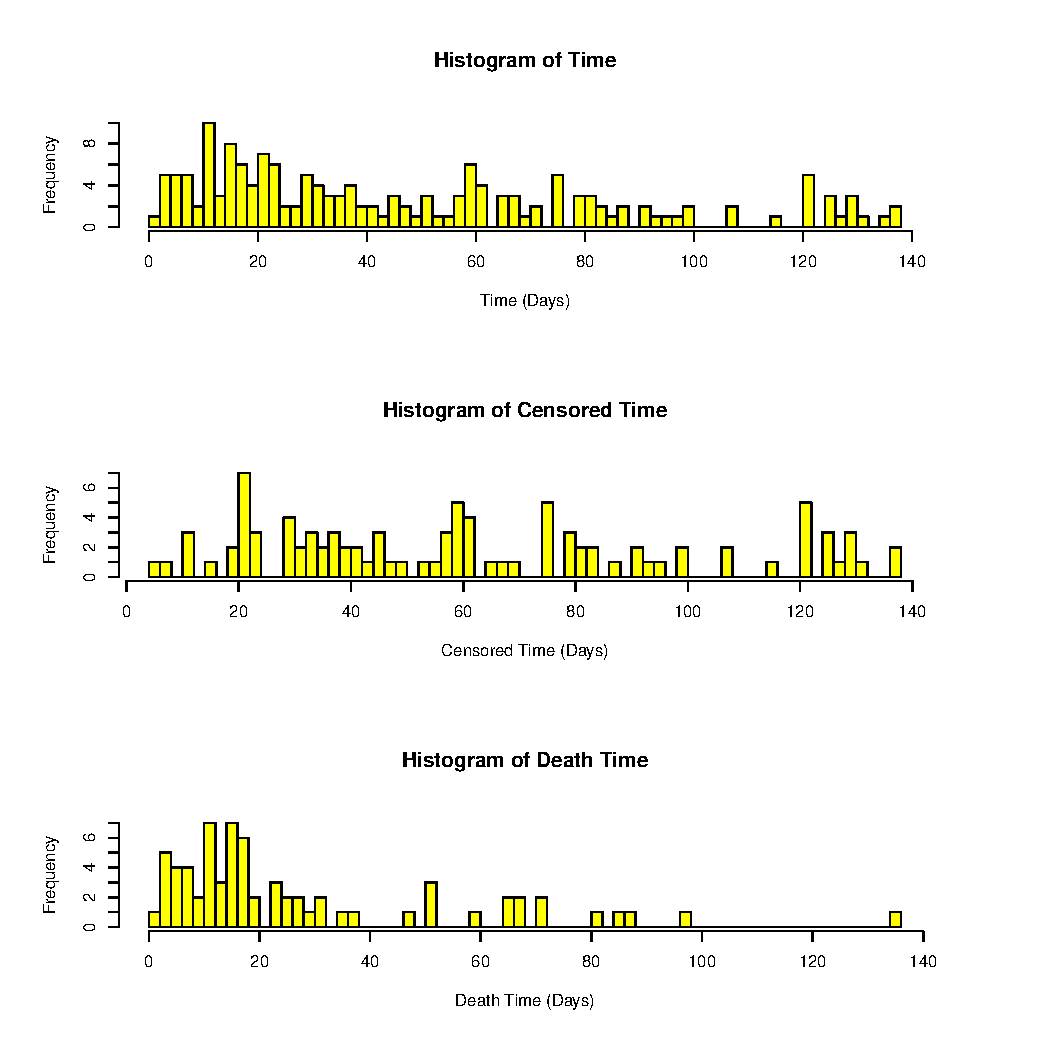
\includegraphics[scale=.4]{raw/times.pdf}
          \caption{\tiny Note: We have more data on lower survival times. And
                               more deaths occurred at lower survival times.}
        \end{figure}
      }

      \frame {
        \frametitle{KM Curve}
        \begin{figure}
          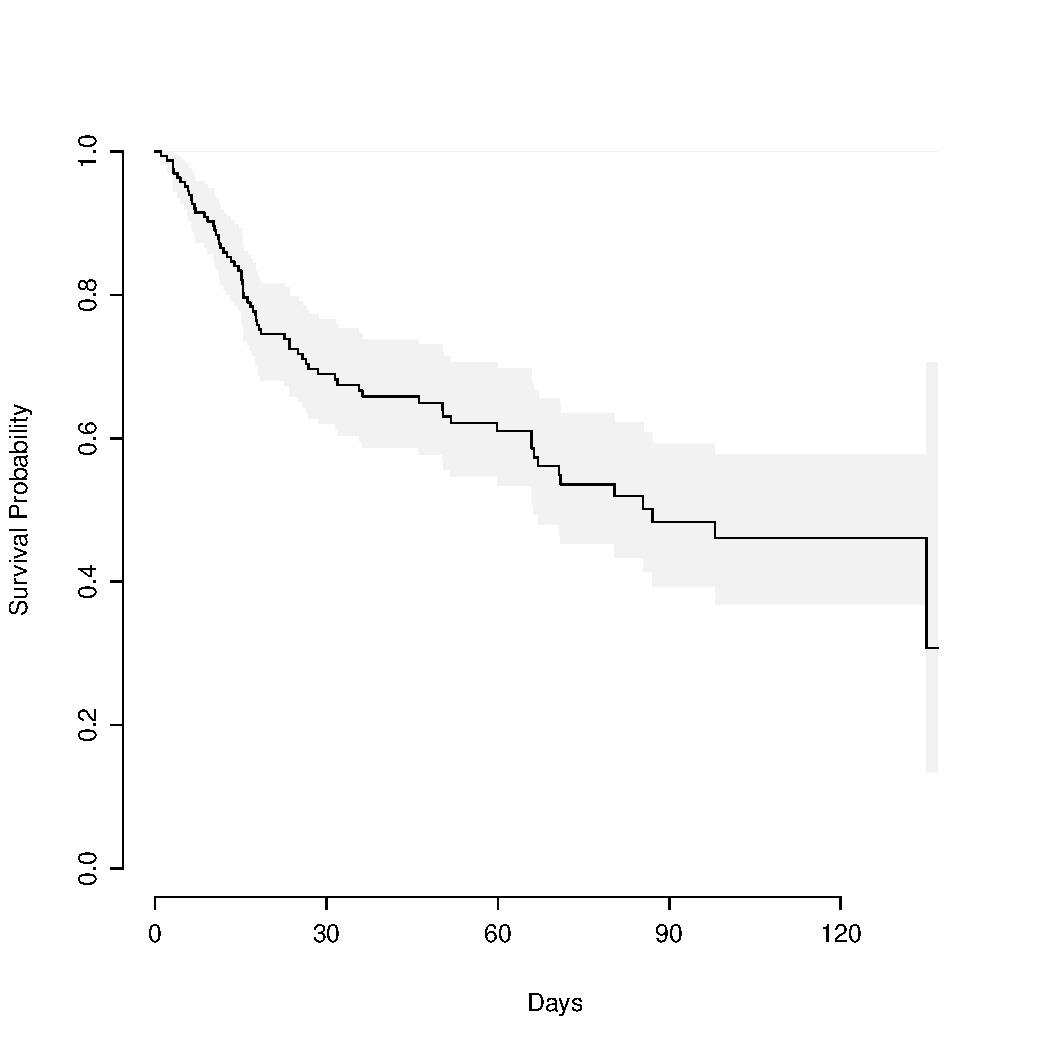
\includegraphics[scale=.3]{raw/KM.pdf}
        \end{figure}
        \tiny Median = 87.07 (33.97, 140.16) 
      }

  \section{False-Positive Discovery Rate}
    %\frame{
    %  \frametitle{FDR}
    %    \begin{enumerate}
    %      \item
    %    \end{enumerate}
    %}
    
    \frame{
      \frametitle{FDR}
         \begin{itemize}
            \item[+] Appropriate for large size of independent and dependent 
                     coefficients
            \item[-] Average fraction of false rejections has to be made
                     or obtained using cross validation
         \end{itemize}
         \wl\wl\wl\wl
         \tiny Interaction terms were not included
    }

    \frame {
      \frametitle{Cox Model Using Variables with FDR $<$ .025}
      \tiny
      % latex table generated in R 3.0.3 by xtable 1.7-1 package
% Mon Apr 21 23:06:25 2014
\begin{table}[ht]
\centering
\begin{tabular}{rrrrrr}
  \hline
 & coef & exp(coef) & se(coef) & z & Pr($>$$|$z$|$) \\ 
  \hline
geneILMN\_1666893 & 0.28 & 1.32 & 0.26 & 1.04 & 0.30 \\ 
  geneILMN\_1689037 & 0.82 & 2.26 & 0.22 & 3.70 & 0.00 \\ 
  geneILMN\_1690017 & 0.32 & 1.37 & 0.28 & 1.15 & 0.25 \\ 
  geneILMN\_1702933 & 0.45 & 1.57 & 0.32 & 1.42 & 0.15 \\ 
  geneILMN\_1714118 & 0.48 & 1.61 & 0.51 & 0.94 & 0.35 \\ 
  geneILMN\_1714592 & -0.15 & 0.86 & 0.37 & -0.40 & 0.69 \\ 
  geneILMN\_1718866 & 0.18 & 1.20 & 0.40 & 0.45 & 0.65 \\ 
  geneILMN\_1745238 & 0.23 & 1.26 & 0.33 & 0.69 & 0.49 \\ 
  geneILMN\_1757351 & 0.00 & 1.00 & 0.16 & 0.03 & 0.98 \\ 
  geneILMN\_1767685 & -0.26 & 0.77 & 0.48 & -0.55 & 0.59 \\ 
  geneILMN\_1807525 & -0.01 & 0.99 & 0.56 & -0.03 & 0.98 \\ 
  geneILMN\_1809336 & 0.40 & 1.49 & 0.28 & 1.42 & 0.15 \\ 
  geneILMN\_1889811 & 0.69 & 2.00 & 0.42 & 1.64 & 0.10 \\ 
   \hline
\end{tabular}
\end{table}

    }

    \frame {
      \frametitle{FDR KM Plots}
      \begin{figure}
        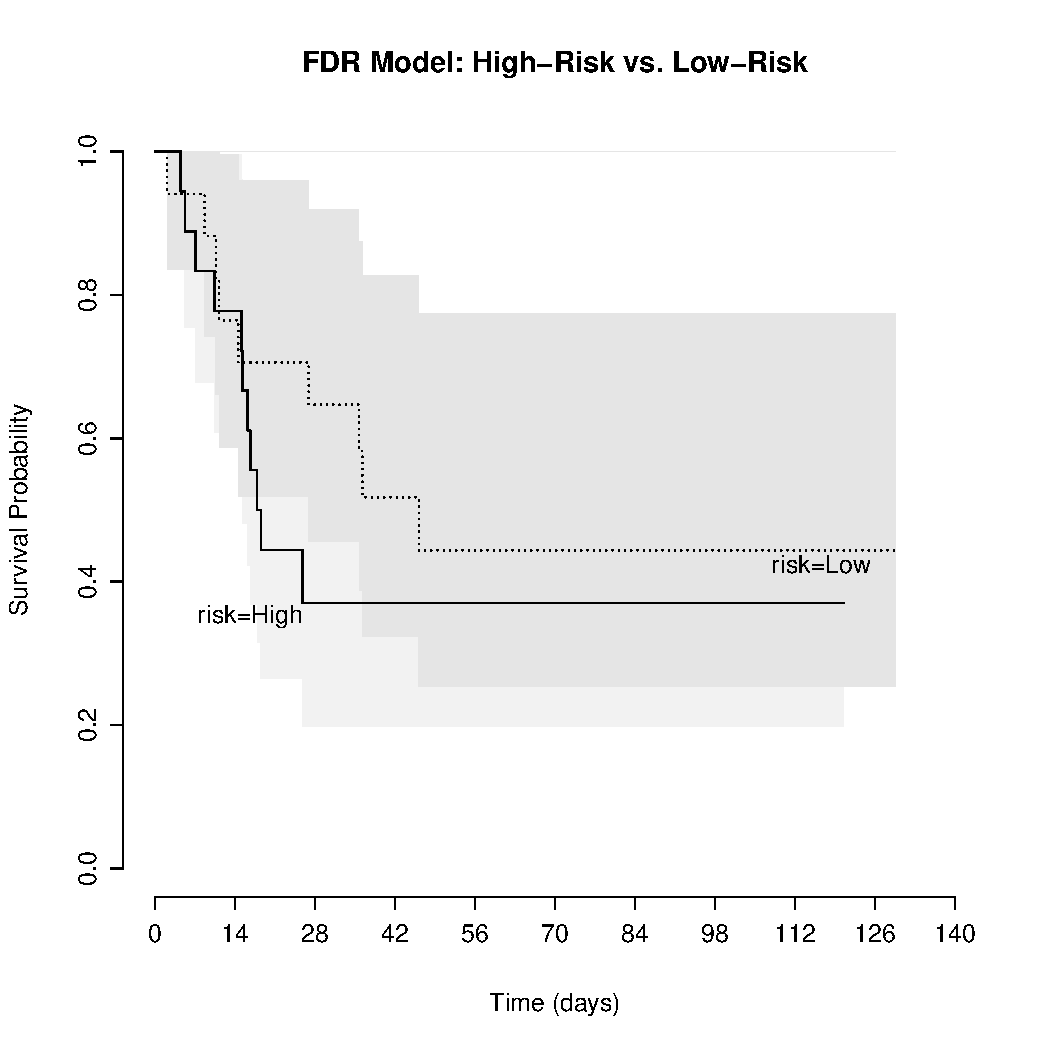
\includegraphics[scale=.3]{raw/fdrKM.pdf}
      \end{figure}
      \tiny Low Median = 18.2. High Median = 46.2 \\
      \tiny Likelihood ratio test=63  on 13 df, p=1.49e-08  n= 130.
    }

    \frame {
      \frametitle{Residuals Plot}
      \begin{figure}
        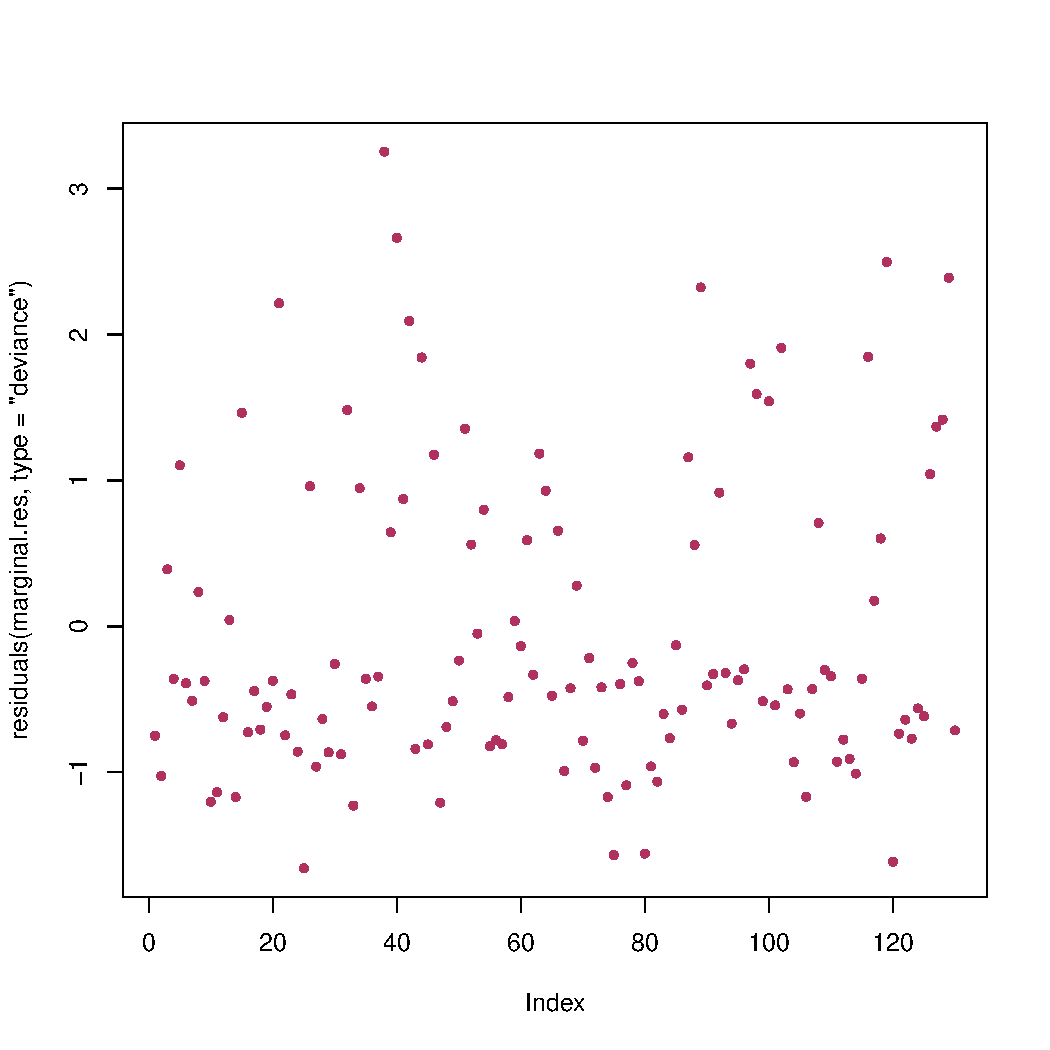
\includegraphics[scale=.4]{raw/fdrResid.pdf}
      \end{figure}  
    }
    
    \frame {
      \frametitle{FDR AUC}
      \begin{figure}
        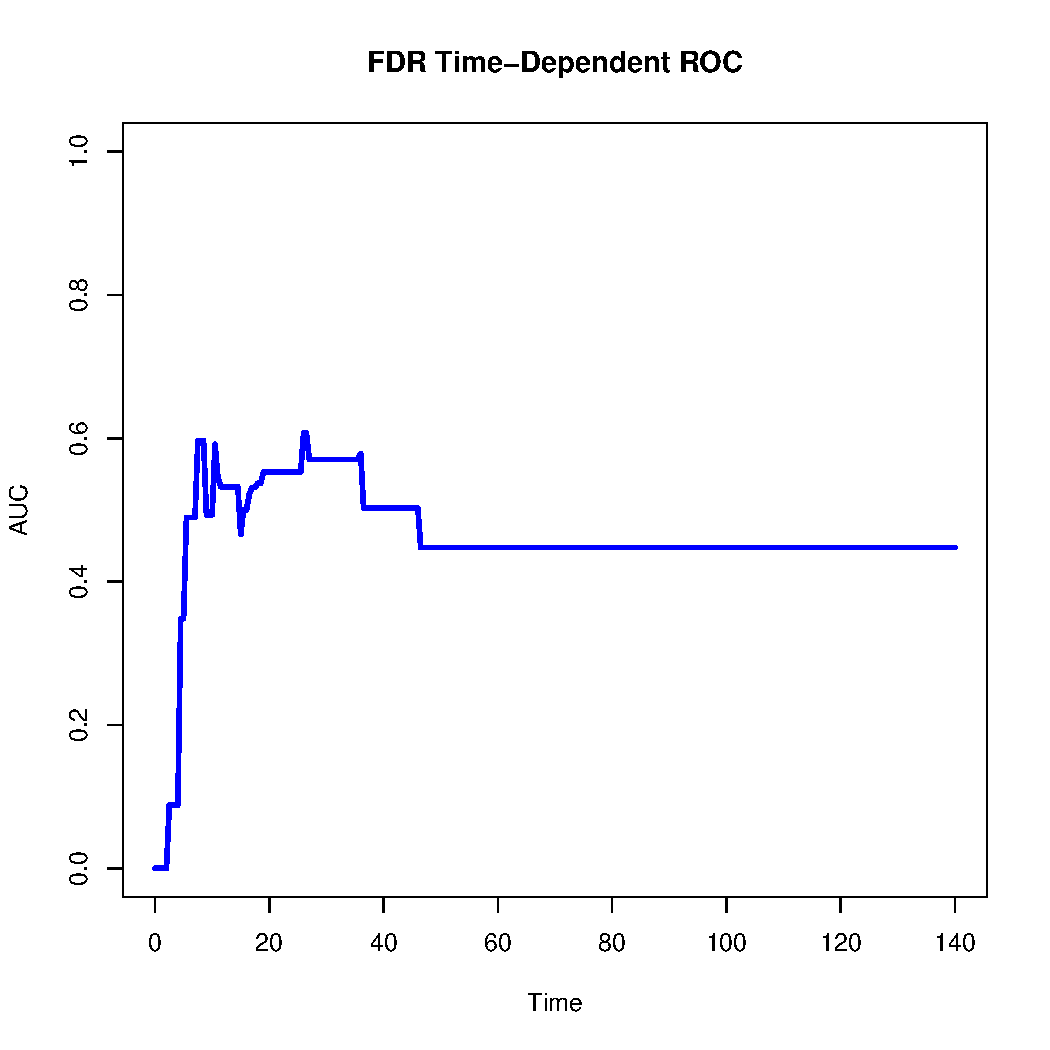
\includegraphics[scale=.4]{raw/fdrAUC.pdf}
      \end{figure}
    }
  

  \section{Lasso}
    %\frame{
    %  \frametitle{Lasso}
    %    \begin{enumerate}
    %      \item
    %    \end{enumerate}
    %}
    
    \frame{
      \frametitle{Lasso}
         \begin{itemize}
            \item[+] Performs model selection 
            \item[-] Tuning parameter needs to be estimated
         \end{itemize}
         \wl\wl\wl\wl
         \tiny Interaction terms were not included
    }

   \frame {
     \frametitle{Selecting Tuning Parameter $\lambda$}
     \begin{figure}
       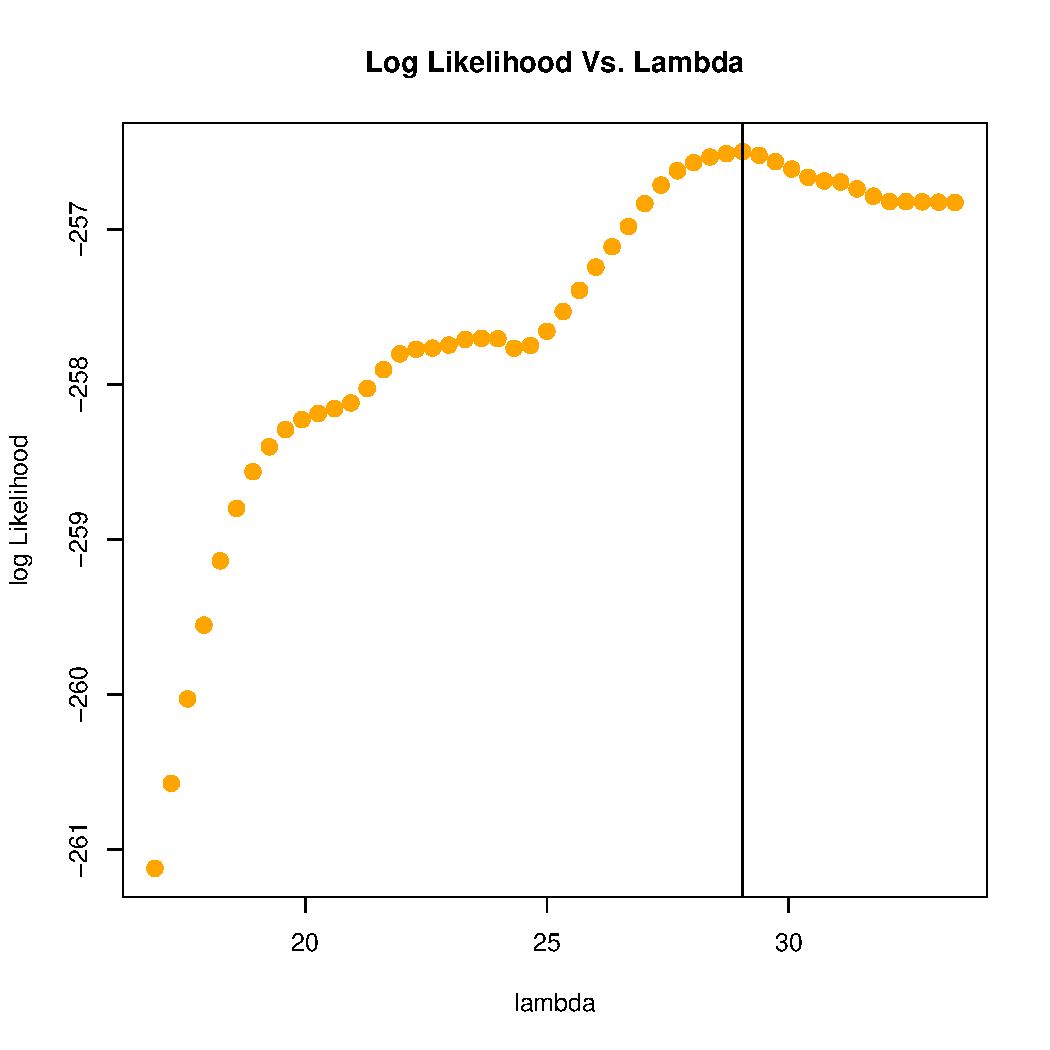
\includegraphics[scale=.4]{raw/logliklamb.pdf}
     \end{figure}
     \tiny $\lambda = 29.95$
   }

  \frame {
    \frametitle{Selected Variables}
    \begin{figure}
      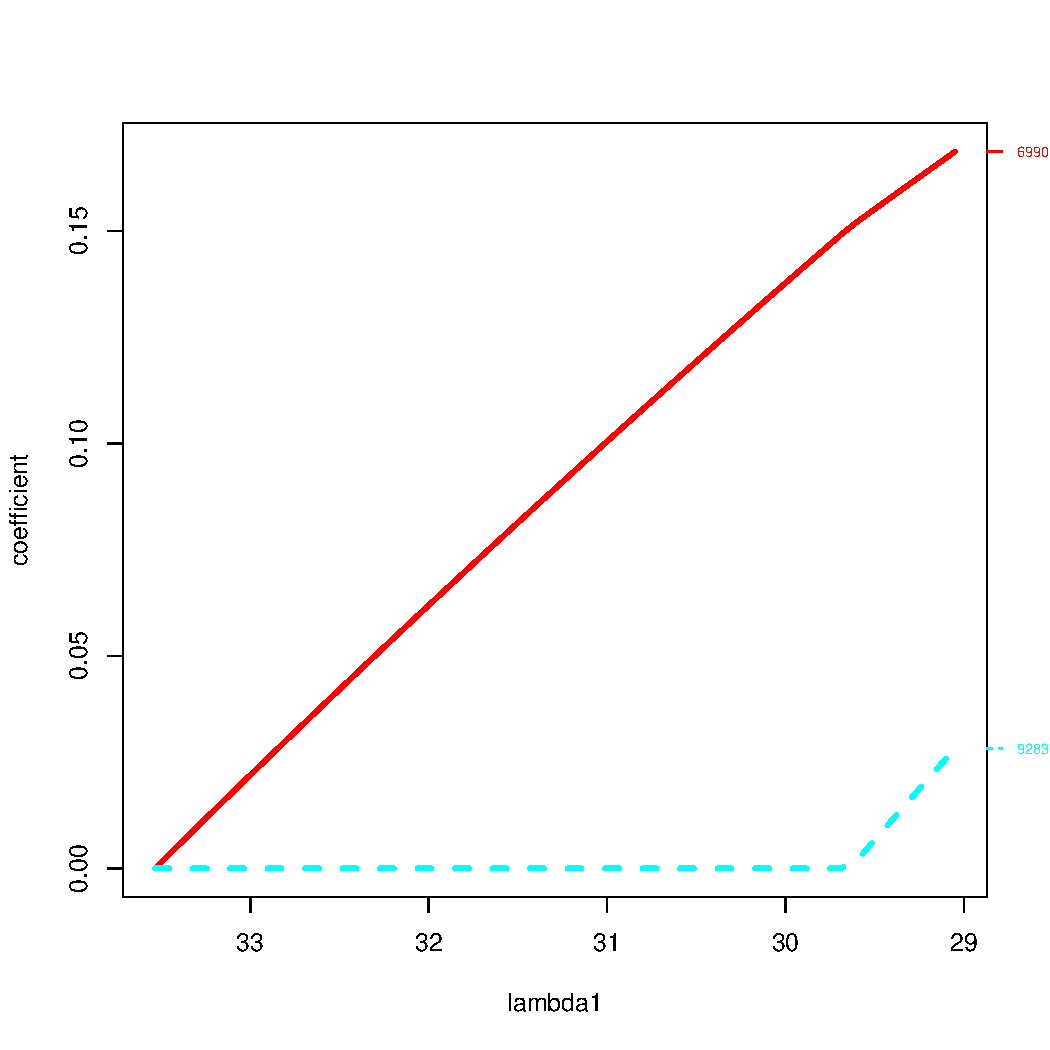
\includegraphics[scale=.3]{raw/selectedVar.pdf}
    \end{figure}
    \tiny
    % latex table generated in R 3.0.3 by xtable 1.7-1 package
% Tue Apr 22 00:10:44 2014
\begin{table}[ht]
\centering
\begin{tabular}{rrr}
  \hline
 & ILMN\_1689037 & ILMN\_1702933 \\ 
  \hline
1 & 0.17 & 0.03 \\ 
   \hline
\end{tabular}
\end{table}

  }
  
  \frame {
    \frametitle{Residuals Plot}
    \begin{figure}
      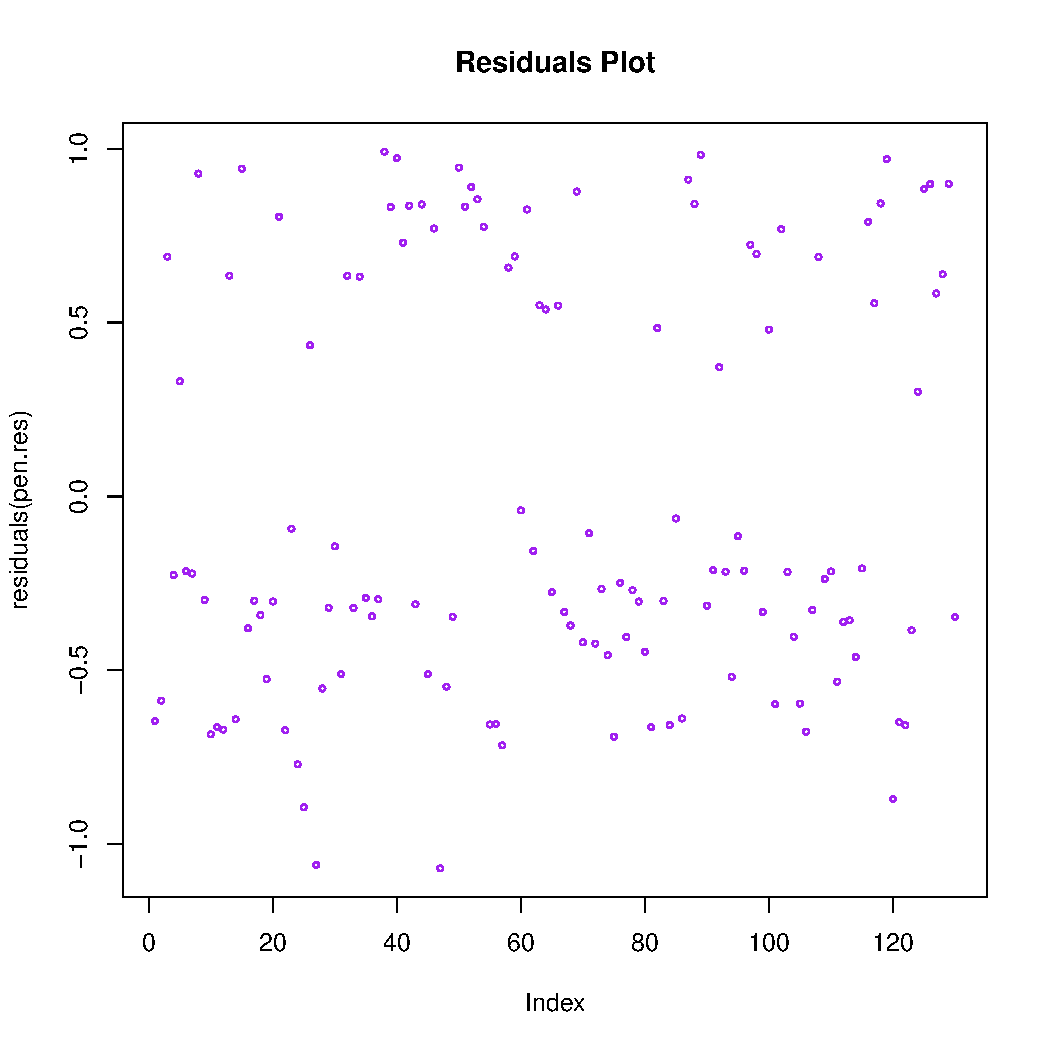
\includegraphics[scale=.4]{raw/lassoResid.pdf}
    \end{figure}
  }


    \frame {
      \frametitle{Lasso KM Plots}
      \begin{figure}
        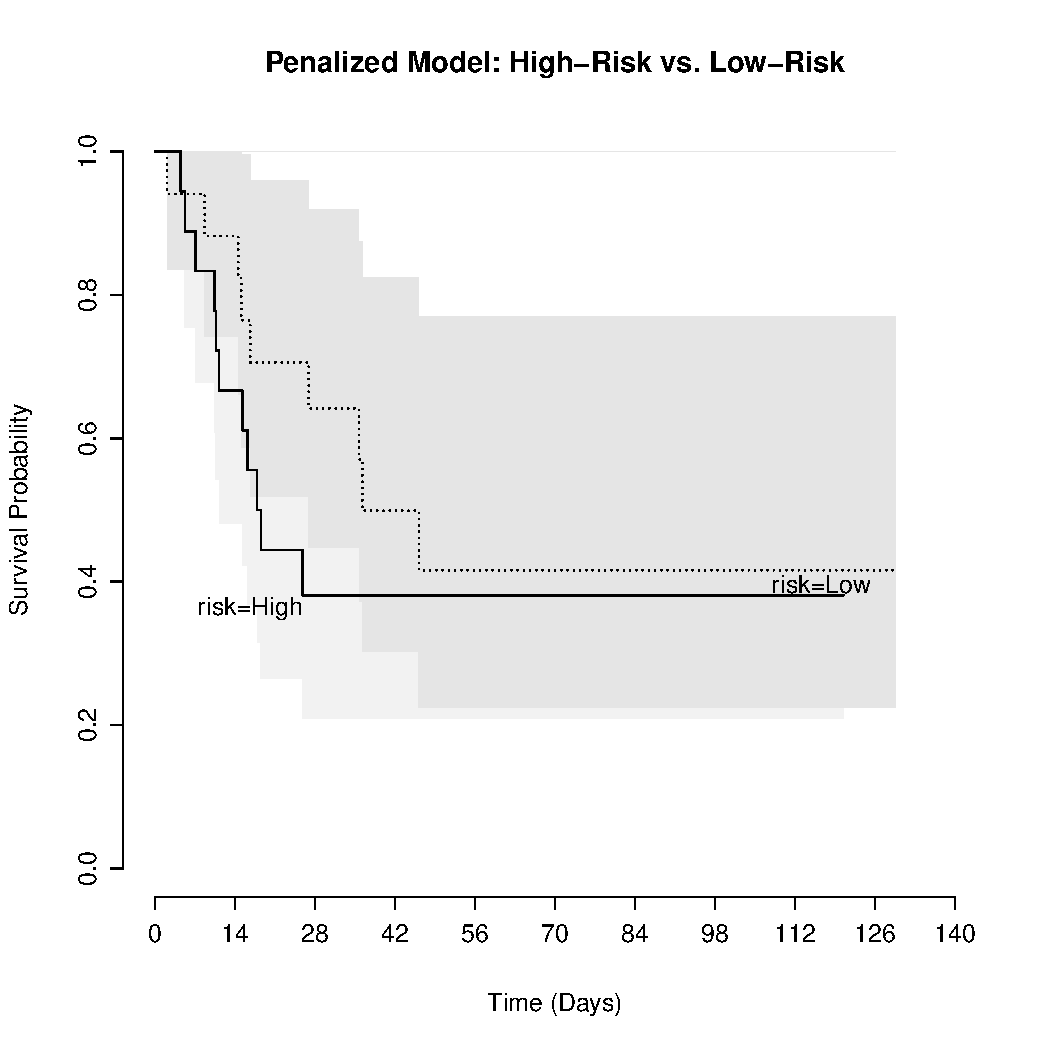
\includegraphics[scale=.3]{raw/lassoKM.pdf}
      \end{figure}
      \tiny Low Median = 36.3 \\
      \tiny High Median = 18.2 \\
      \tiny Likelihood ratio test=41.9  on 2 df, p=7.83e-10
    }

    \frame {
      \frametitle{Lasso AUC}
      \begin{figure}
        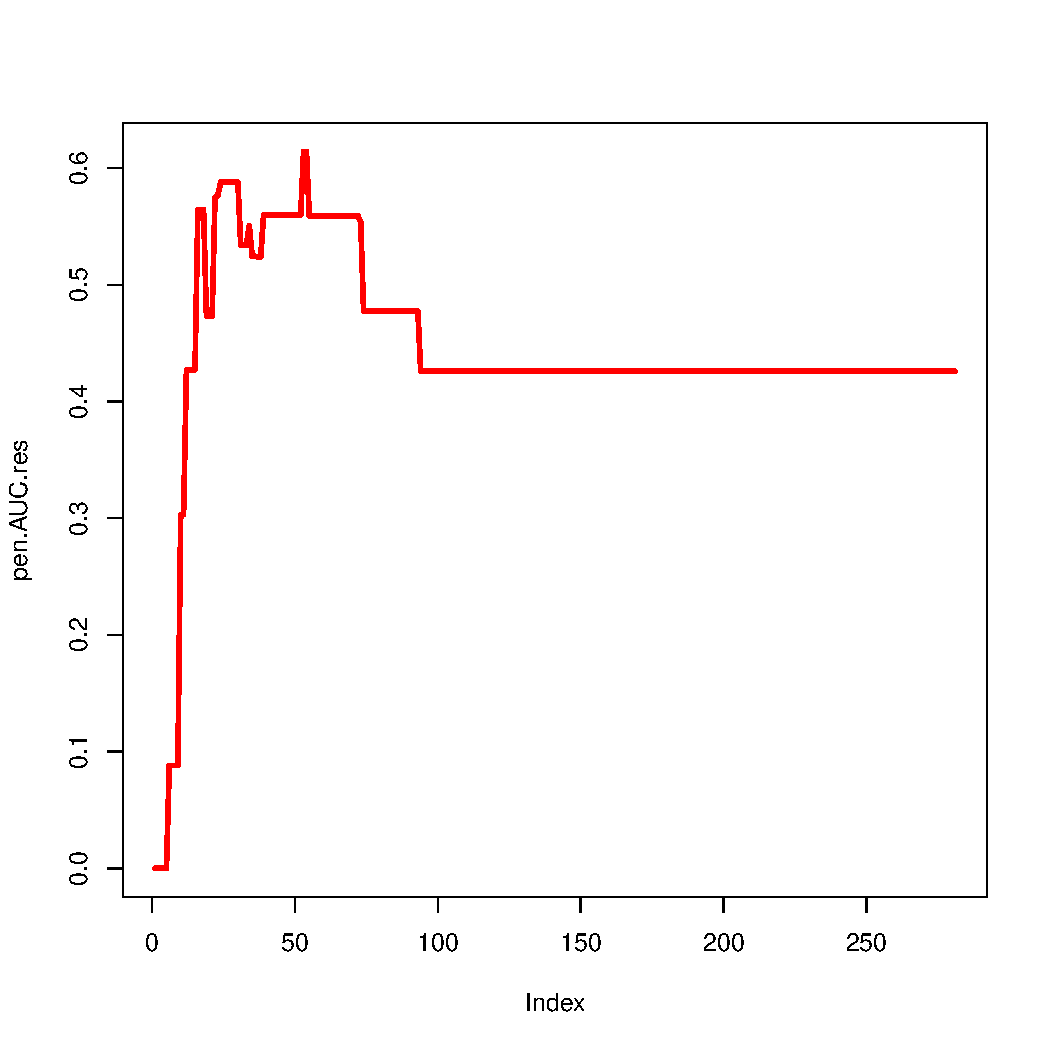
\includegraphics[scale=.4]{raw/lassoAUC.pdf}
      \end{figure}
    }

   
  \section{Random Forests}
    \frame{
      \frametitle{Random Forests Model}
        \begin{enumerate}
          \item A regression tree is a model that predicts the response of an input
                based on a sequence of decisions
          \item A Random Forest is created from many trees
          \item The predicted response of the random forest is the mean of 
                the predictions of the individual trees
        \end{enumerate}
    }
    
    \frame{
      \frametitle{Random Forest}
         \begin{itemize}
            \item[+] Good for modelling non-linear data \\
                     (data assumed to be nonlinear)
            \item[-] Lower prediction accuracy
         \end{itemize}
         \wl\wl\wl\wl
         \tiny Interaction terms were not included
    }

    \frame{
      \frametitle{Variable Importance}
      \begin{figure}
        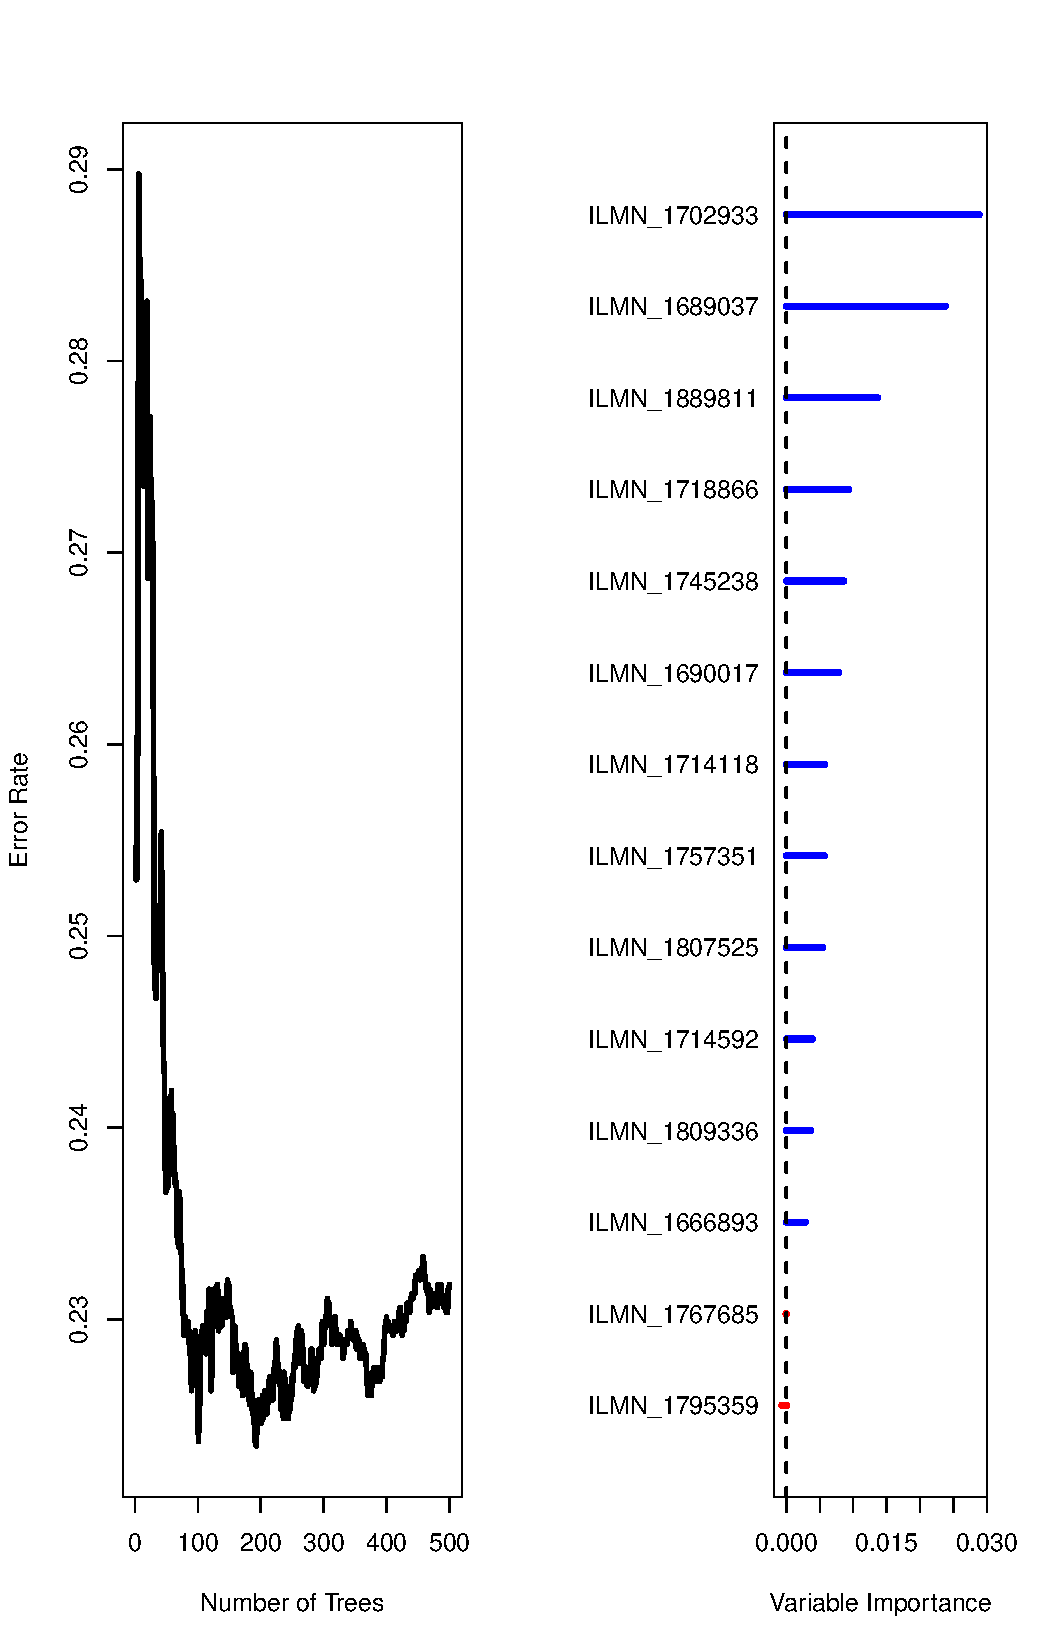
\includegraphics[scale=.275]{raw/varImp.pdf}
      \end{figure}
    } 

    \frame {
      \frametitle{Cox Model Using Important Variables from Random Forest}
      \small
      % latex table generated in R 3.0.3 by xtable 1.7-1 package
% Mon Apr 21 14:32:50 2014
\begin{table}[ht]
\centering
\begin{tabular}{rrrrrr}
  \hline
 & coef & exp(coef) & se(coef) & z & p \\ 
  \hline
genesILMN\_1689037 & 0.68 & 1.98 & 0.18 & 3.70 & 0.00 \\ 
  genesILMN\_1702933 & 1.03 & 2.80 & 0.25 & 4.08 & 0.00 \\ 
  genesILMN\_1704154 & 0.32 & 1.37 & 0.19 & 1.69 & 0.09 \\ 
  genesILMN\_1749989 & -2.32 & 0.10 & 1.33 & -1.74 & 0.08 \\ 
   \hline
\end{tabular}
\end{table}
\wl
\tiny Likelihood ratio test=49.5  on 4 df, p=4.58e-10  n= 130, number of events= 49



    }

    \frame{
      \frametitle{Random Forest KM Plots}
      \tiny Important Markers: 
            ILMN\_1689037, ILMN\_1702933, ILMN\_1704154, ILMN\_1749989 
      \begin{figure}
        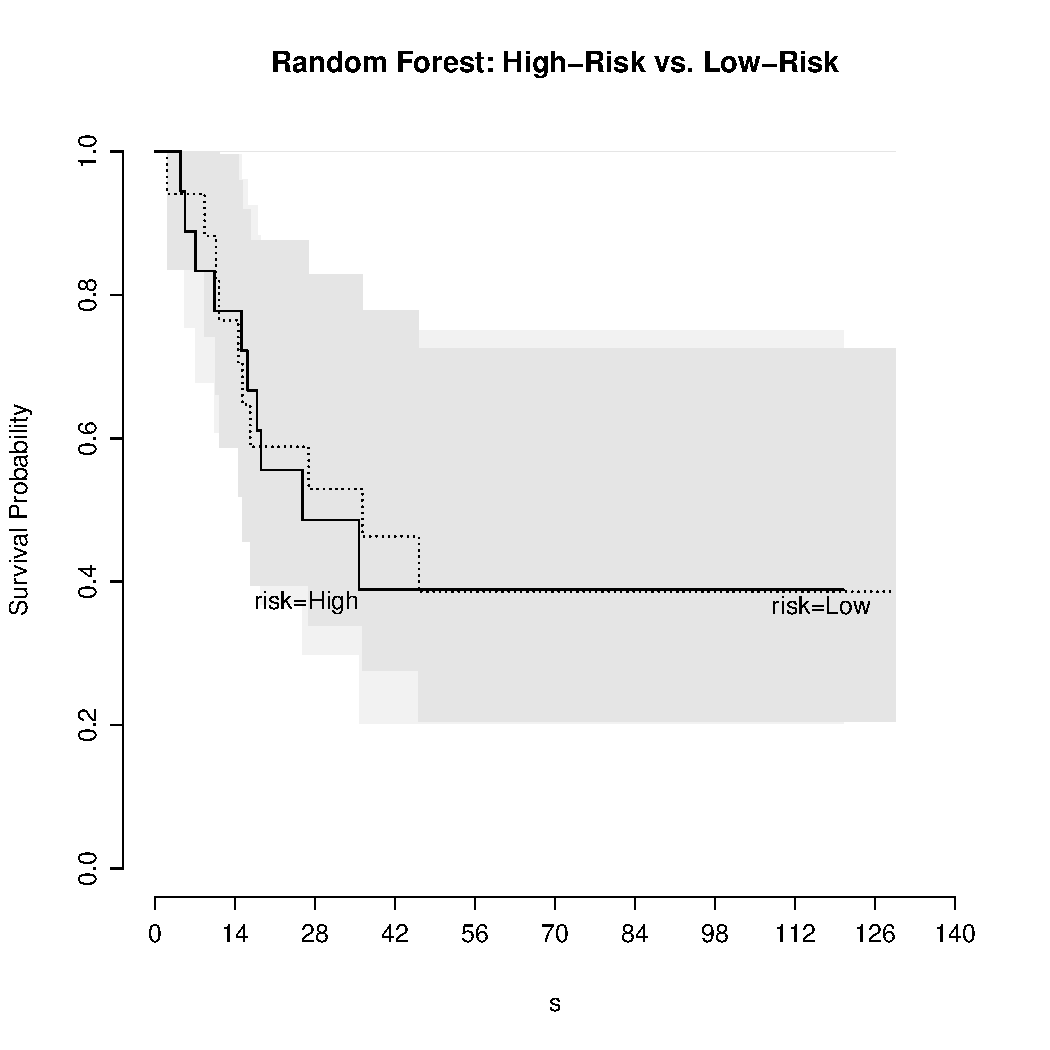
\includegraphics[scale=.3]{raw/treeKM.pdf}
      \end{figure}
      \tiny % latex table generated in R 3.0.3 by xtable 1.7-1 package
% Mon Apr 21 15:10:45 2014
\begin{table}[ht]
\centering
\caption{\tiny Median} 
\begin{tabular}{rrrr}
  \hline
 & Estimate & CI.Lower & CI.Upper \\ 
  \hline
Low-Risk Group & 36.30 & -39.43 & 112.03 \\ 
  High-Risk Group & 25.83 & -9.78 & 61.45 \\ 
   \hline
\end{tabular}
\end{table}

      \tiny Likelihood Ratio Test = 0.02  on 1 df,   p=0.8958 (Curves similar)
    }

    \frame {
      \frametitle{Residuals Plot}
      \begin{figure}
        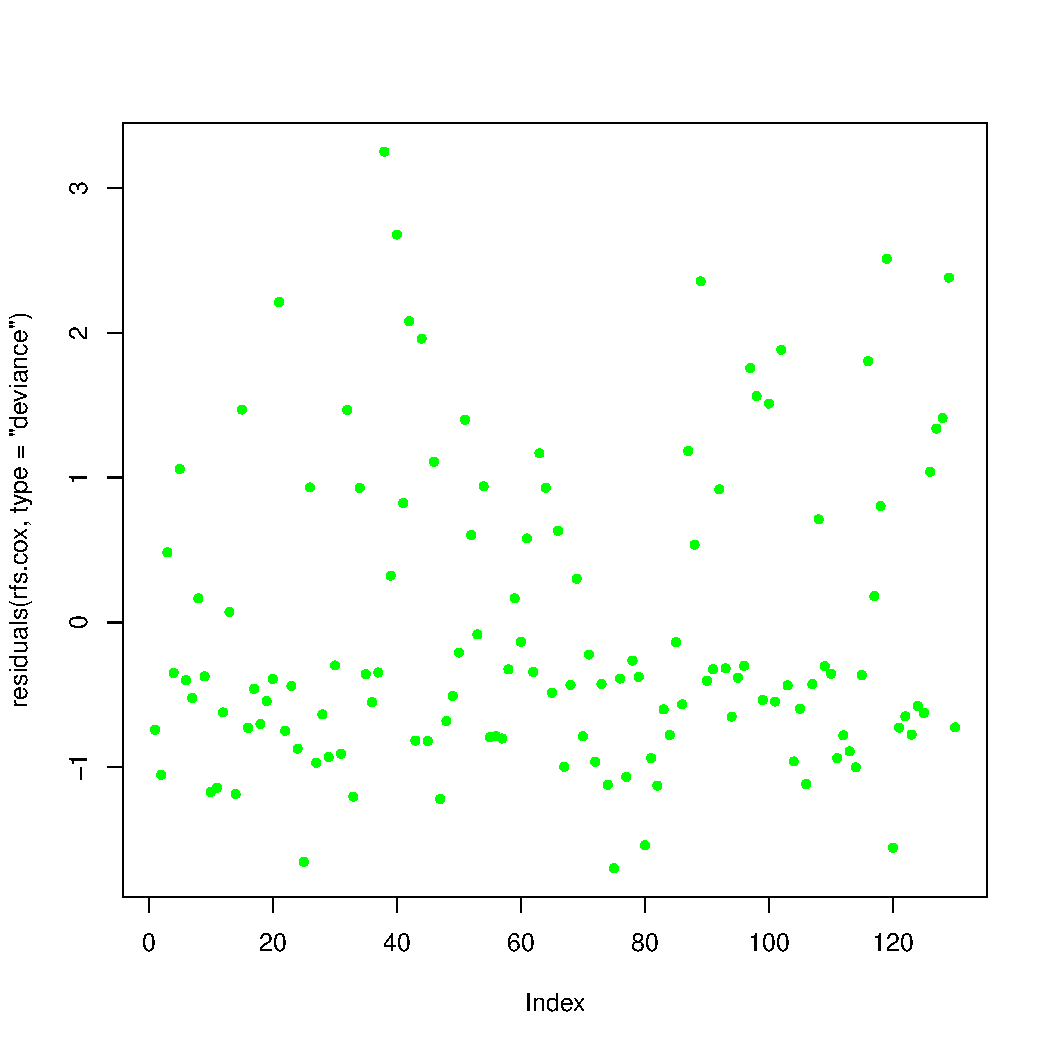
\includegraphics[scale=.4]{raw/rfResid.pdf}
      \end{figure}
    }

    \frame {
      \frametitle{Random Forest AUC}
      \begin{figure}
        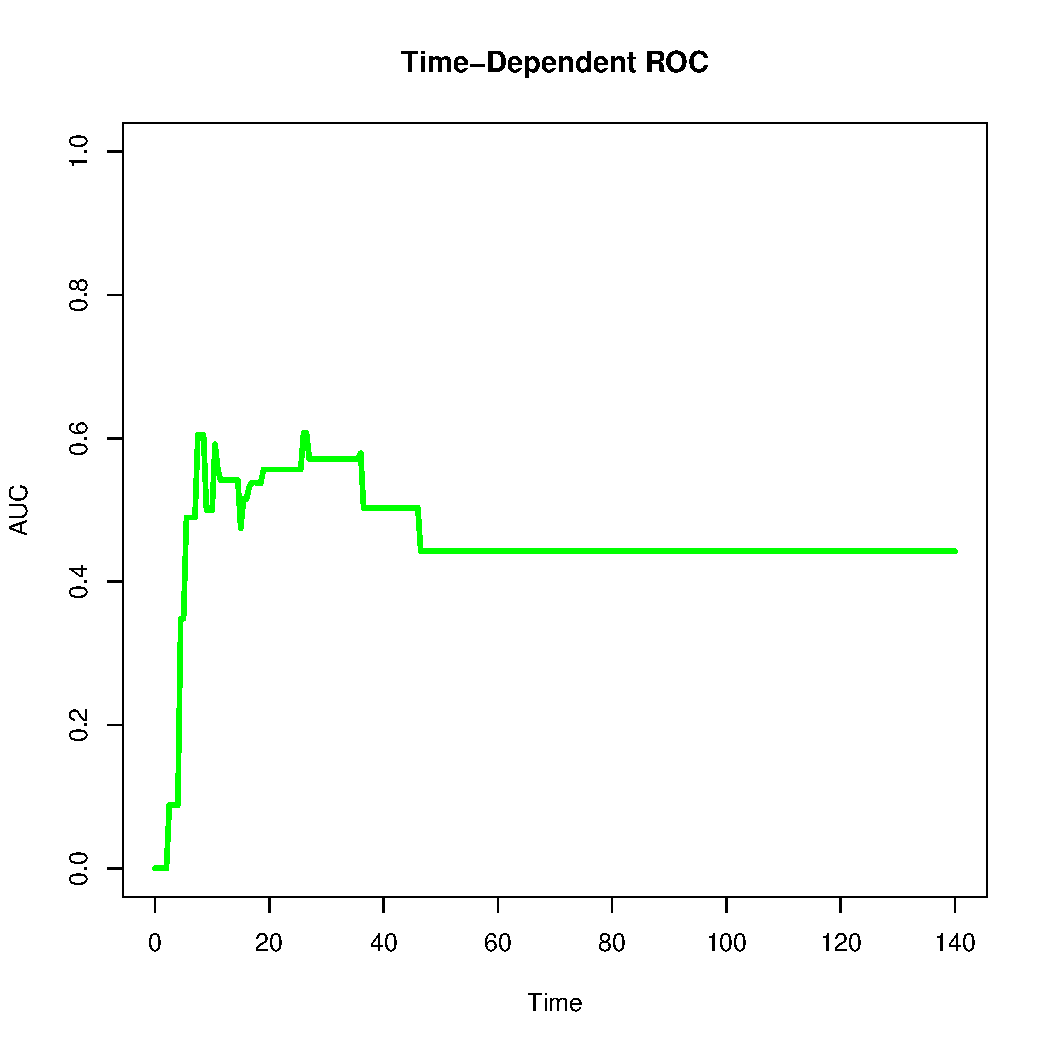
\includegraphics[scale=.4]{raw/rfAUC.pdf}
      \end{figure}
    }


  \section{Hierarchical Clustering}
    \frame{
      \frametitle{Hierarchical Clustering Model}
        \begin{enumerate}
          \item Identify hyperplane that provides maximum separation between clusters
        \end{enumerate}
    }
    
    \frame{
      \frametitle{Hierarchical Clustering}
         \begin{itemize}
            \item[+] Good result visualization
            \item[+] Will obtain a hierarchy of clusters
            \item[+] Fast computation
            \item[+] Helpful for identifying gene expression data patterns in time
                     and space
            \item[-] Doesn't identify best clusters
            \item[-] Sensitive to noise and outliers
            \item[-] Might break for large clusters

         \end{itemize}
         \wl\wl\wl\wl
         \tiny Interaction terms were not included
    }
    
    \frame {
      \frametitle{H-Clust model}
      \begin{figure}
        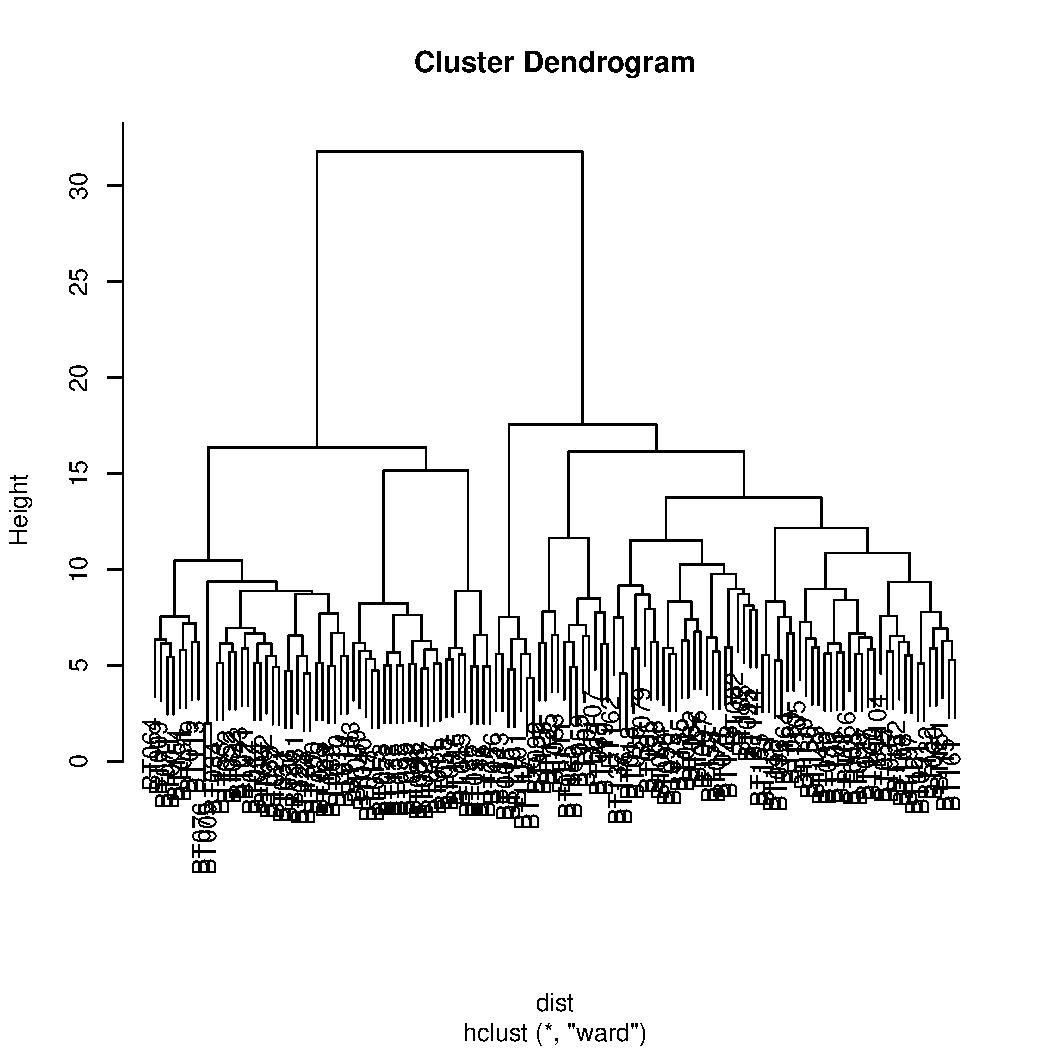
\includegraphics[scale=.4]{raw/ward.pdf}
      \end{figure}
    }

    \frame {
      \frametitle{Cox Model Using Important Variables from H-Clust}
      \small
      % latex table generated in R 3.0.3 by xtable 1.7-1 package
% Mon Apr 21 18:09:12 2014
\begin{table}[ht]
\centering
\begin{tabular}{rrrrrr}
  \hline
 & coef & exp(coef) & se(coef) & z & p \\ 
  \hline
genesILMN\_1651236 & -0.19 & 0.83 & 0.41 & -0.45 & 0.65 \\ 
  genesILMN\_1651260 & 0.44 & 1.55 & 0.38 & 1.16 & 0.25 \\ 
  genesILMN\_1651429 & 0.26 & 1.29 & 0.14 & 1.78 & 0.08 \\ 
  genesILMN\_1651433 & -0.02 & 0.98 & 0.35 & -0.05 & 0.96 \\ 
  genesILMN\_1651438 & 0.47 & 1.60 & 0.29 & 1.65 & 0.10 \\ 
  genesILMN\_1651557 & -0.23 & 0.80 & 0.25 & -0.92 & 0.36 \\ 
  genesILMN\_1651574 & -0.24 & 0.78 & 0.11 & -2.21 & 0.03 \\ 
  genesILMN\_1651611 & 0.17 & 1.19 & 0.16 & 1.04 & 0.30 \\ 
  genesILMN\_1651652 & -0.42 & 0.66 & 0.32 & -1.31 & 0.19 \\ 
  genesILMN\_1651694 & 0.32 & 1.38 & 0.25 & 1.27 & 0.20 \\ 
  genesILMN\_1651799 & 0.24 & 1.27 & 0.20 & 1.18 & 0.24 \\ 
   \hline
\end{tabular}
\end{table}

      \tiny (p-value $< 10^{-5}$)
    }
    
    \frame {
      \frametitle{Plot of Deviance Residuals}
      \begin{figure}
        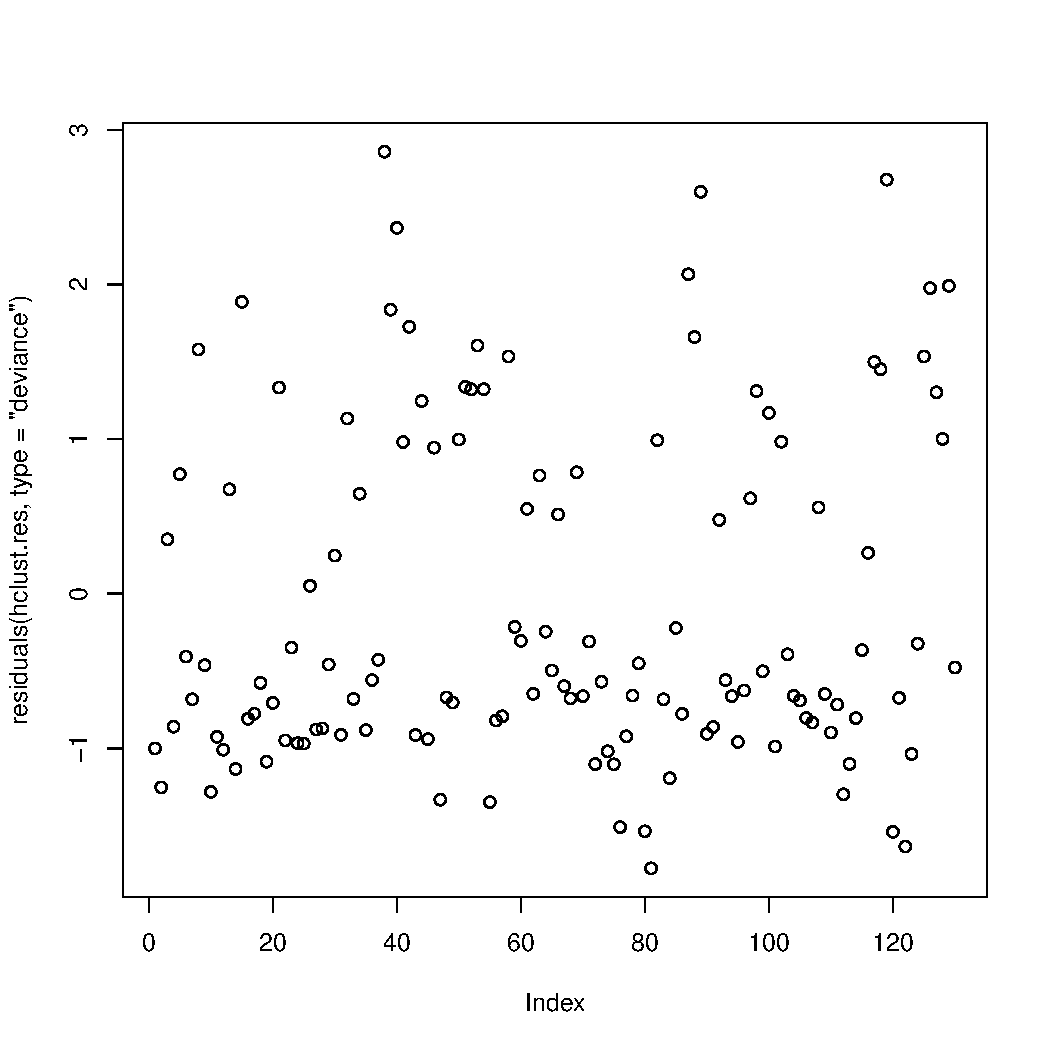
\includegraphics[scale=.4]{raw/devResTree.pdf}
      \end{figure}
    }

    \frame{
      \frametitle{H-Clust KM Plots}
      \begin{figure}
        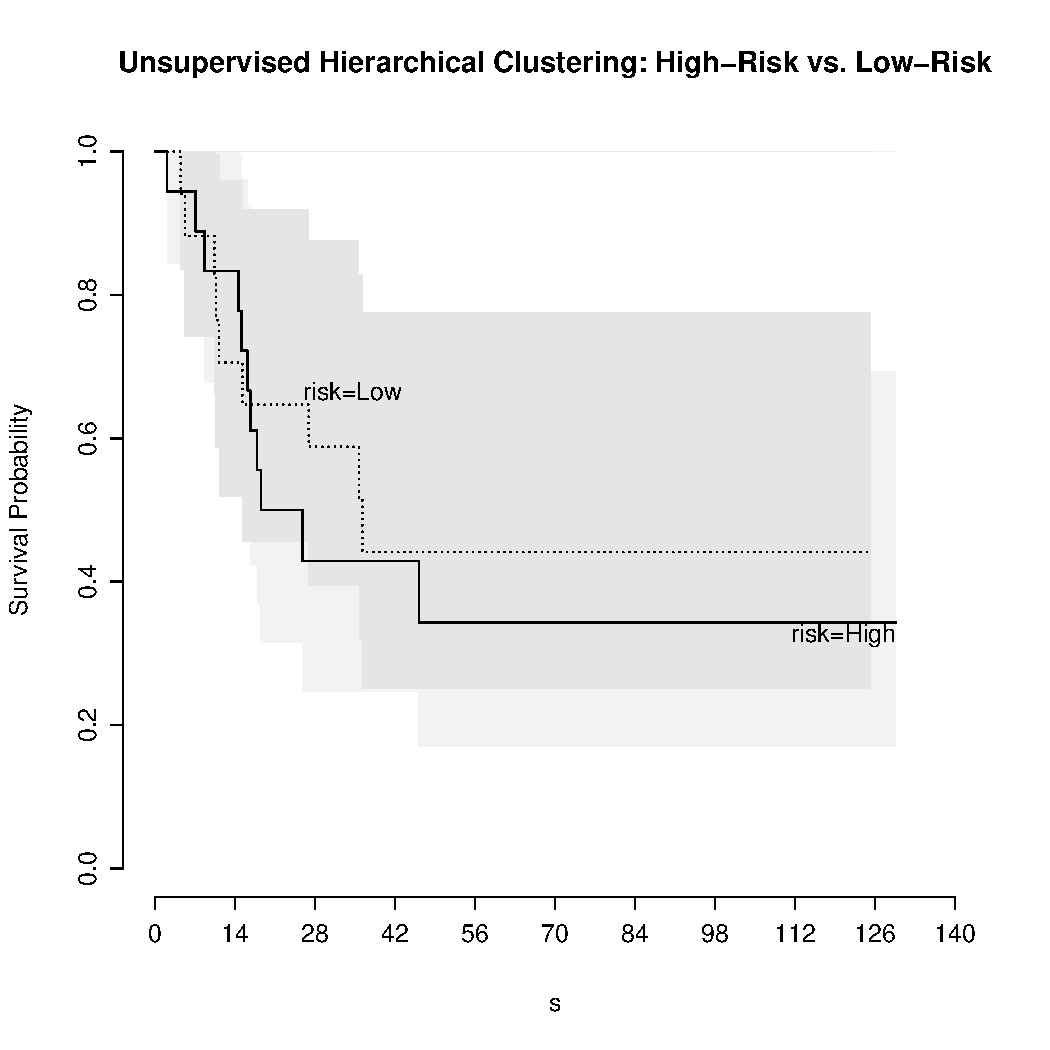
\includegraphics[scale=.3]{raw/clustKM.pdf}
      \end{figure}
      \tiny Low Risk Median = 36.3 (23.1, 49.5)\\
      \tiny High Risk Median = 25.8\\
      \tiny Likelihood ratio test= 22.25 on 11 df.  p-value=0.0225 \\
    }
    
    \frame {
      \frametitle{H-Clust AUC}
      \begin{figure}
        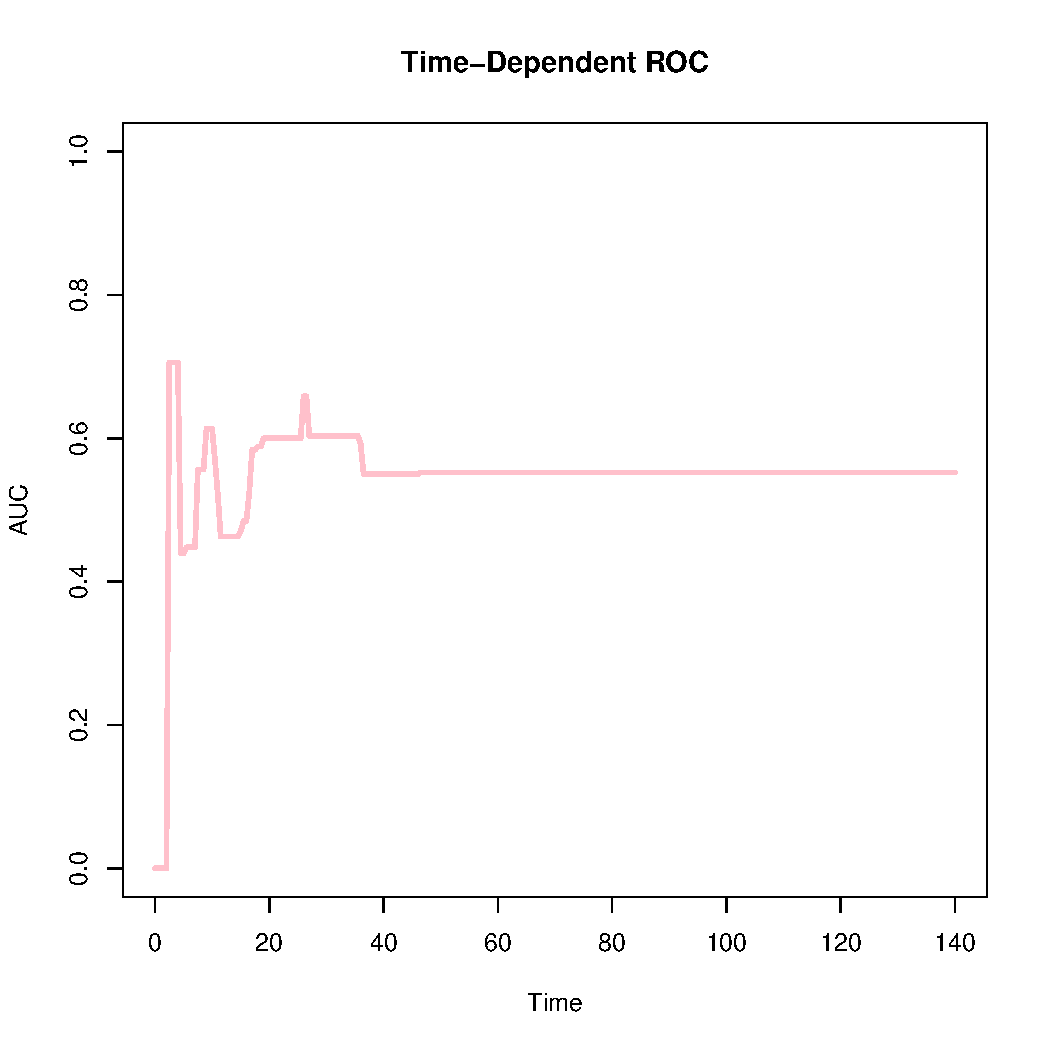
\includegraphics[scale=.4]{raw/clustAUC.pdf}
      \end{figure}
    }

  \section{Principal Component Analysis}
    \frame{
      \frametitle{Principal Component Analysis (PCA)}
        \begin{enumerate}
          \item Orthogonal Transformation
          \item Convert a set of observations of possibly correlated variables 
                into a set of values of linearly uncorrelated variables
        \end{enumerate}
    }
    
    \frame{
      \frametitle{PCA}
         \begin{itemize}
            \item[+] Lack of redundancy of data
            \item[+] Reduced complexity 
            \item[+] Smaller database representation
            \item[+] Reduced noise b/c the maximum variation basis is chosen (small variations are ignored)
            \item[-] The covariance matrix is hard to evaluate
            \item[-] Ability to capture variance depends on the training data 
         \end{itemize}
         \wl\wl\wl\wl
         \tiny Interaction terms were not included
    }

    \frame{
      \frametitle{PCA LRT Threshold}
      \begin{figure}
        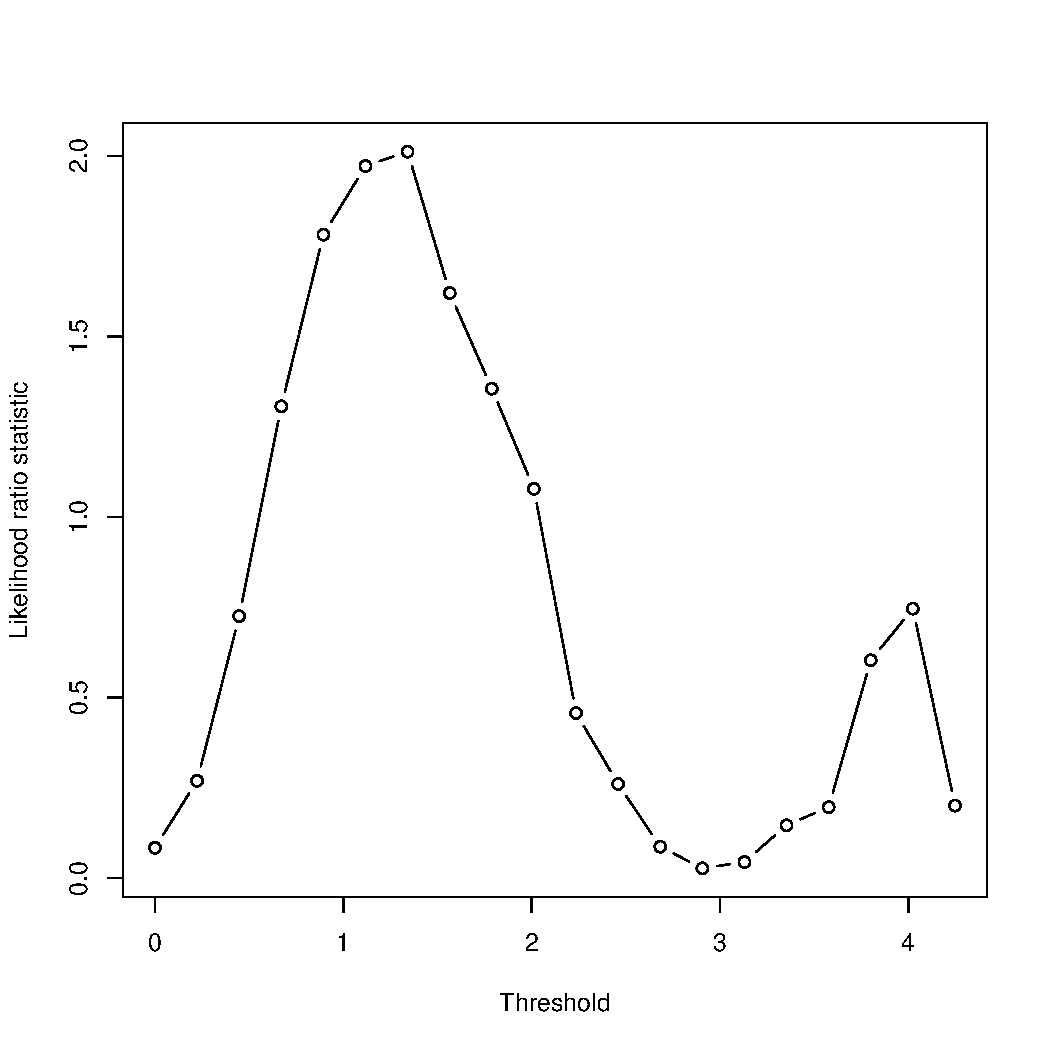
\includegraphics[scale=.4]{raw/superpcLR.pdf}
      \end{figure}
      \tiny threshold $\approx$ 1.34
    }  

    \frame {
      \frametitle{Cox Model Using Principal Components}
      \tiny
      % latex table generated in R 3.0.3 by xtable 1.7-1 package
% Mon Apr 21 19:20:27 2014
\begin{table}[ht]
\centering
\begin{tabular}{rrrrrr}
  \hline
 & coef & exp(coef) & se(coef) & z & Pr($>$$|$z$|$) \\ 
  \hline
geneILMN\_1651574 & -0.17 & 0.84 & 0.13 & -1.37 & 0.17 \\ 
  geneILMN\_1651429 & 0.23 & 1.25 & 0.21 & 1.08 & 0.28 \\ 
  geneILMN\_1651237 & -0.27 & 0.77 & 0.20 & -1.32 & 0.19 \\ 
  geneILMN\_1651611 & -0.07 & 0.93 & 0.16 & -0.46 & 0.65 \\ 
  geneILMN\_1651832 & -0.19 & 0.82 & 0.35 & -0.55 & 0.58 \\ 
  geneILMN\_1651428 & 0.16 & 1.18 & 0.27 & 0.60 & 0.55 \\ 
  geneILMN\_1651496 & 0.02 & 1.02 & 0.23 & 0.10 & 0.92 \\ 
  geneILMN\_1651776 & 0.23 & 1.26 & 0.32 & 0.70 & 0.48 \\ 
  geneILMN\_1651745 & -0.51 & 0.60 & 0.23 & -2.24 & 0.02 \\ 
  geneILMN\_1651364 & 0.39 & 1.48 & 0.38 & 1.03 & 0.30 \\ 
  geneILMN\_1651789 & 0.46 & 1.58 & 0.22 & 2.07 & 0.04 \\ 
  geneILMN\_1651538 & 0.02 & 1.02 & 0.36 & 0.05 & 0.96 \\ 
  geneILMN\_1651872 & 0.74 & 2.09 & 0.39 & 1.90 & 0.06 \\ 
  geneILMN\_1651254 & -1.15 & 0.32 & 0.44 & -2.61 & 0.01 \\ 
  geneILMN\_1651336 & -0.43 & 0.65 & 0.52 & -0.83 & 0.41 \\ 
  geneILMN\_1651544 & -0.97 & 0.38 & 0.40 & -2.42 & 0.02 \\ 
  geneILMN\_1651375 & 0.30 & 1.35 & 0.27 & 1.09 & 0.28 \\ 
  geneILMN\_1651517 & -1.59 & 0.20 & 0.88 & -1.82 & 0.07 \\ 
   \hline
\end{tabular}
\end{table}

      \tiny Likelihood ratio test=3.76  on 3 df, p=0.288  n= 35

    }
    
    \frame{
      \frametitle{PCA KM Plots}
      \begin{figure}
        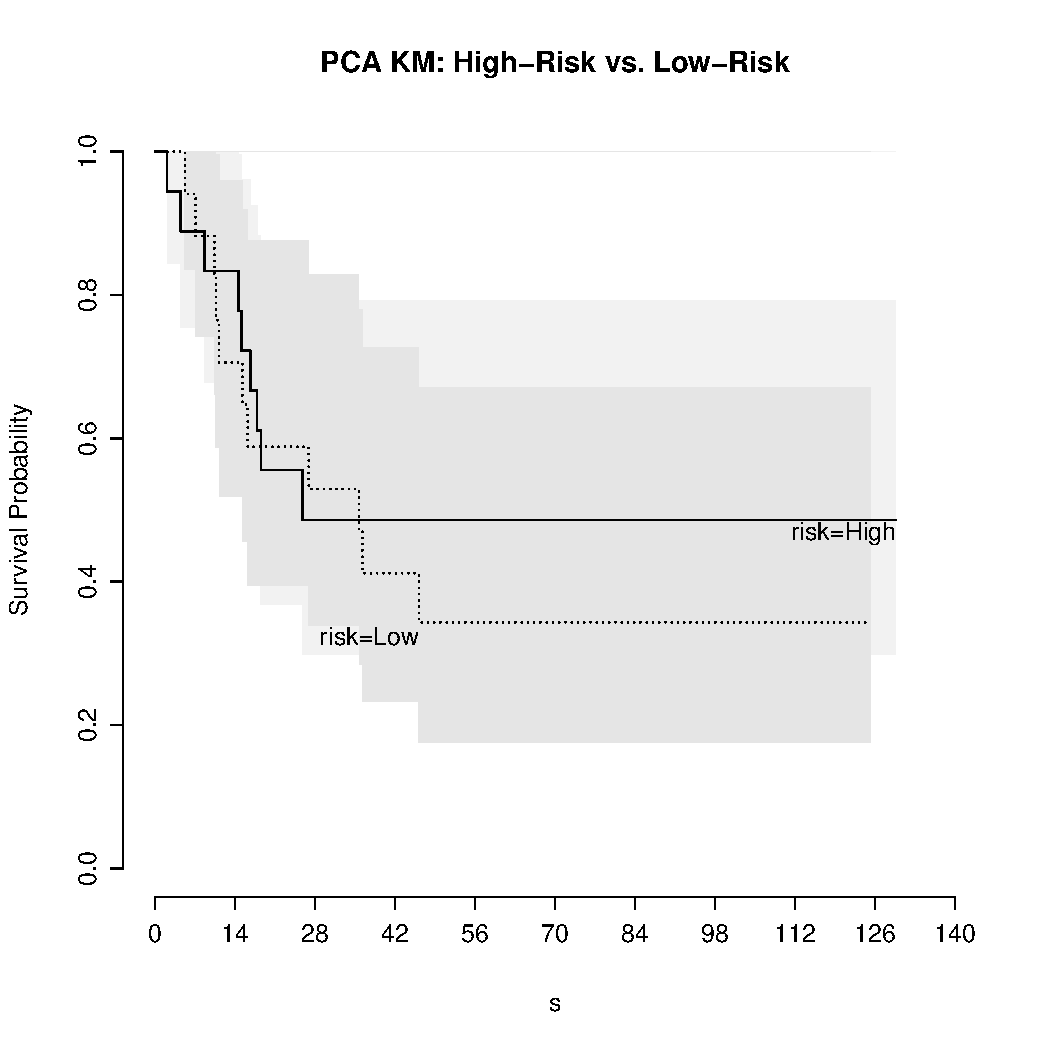
\includegraphics[scale=.3]{raw/pcaKM.pdf}
      \end{figure}
      \tiny Low Risk Group Median = 35.7. High Risk Group Median = 25.8.\\
      \tiny Likelihood ratio test=59.8  on 18 df, p=2.21e-06
    }

    \frame {
      \frametitle{Plot of Deviance Residuals}
      \begin{figure}
        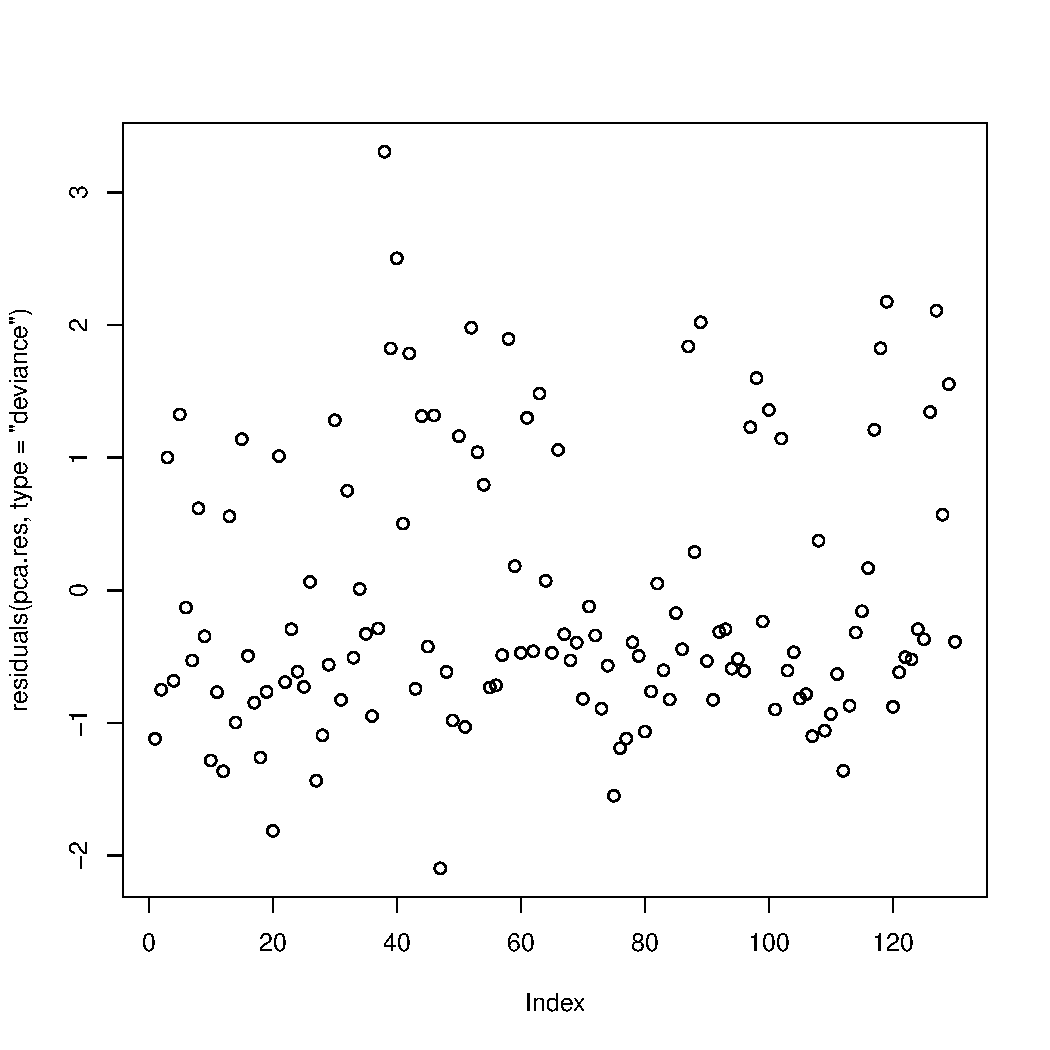
\includegraphics[scale=.4]{raw/devResPCA.pdf}
      \end{figure}
    }
    
    \frame {
      \frametitle{PCA AUC}
      \begin{figure}
        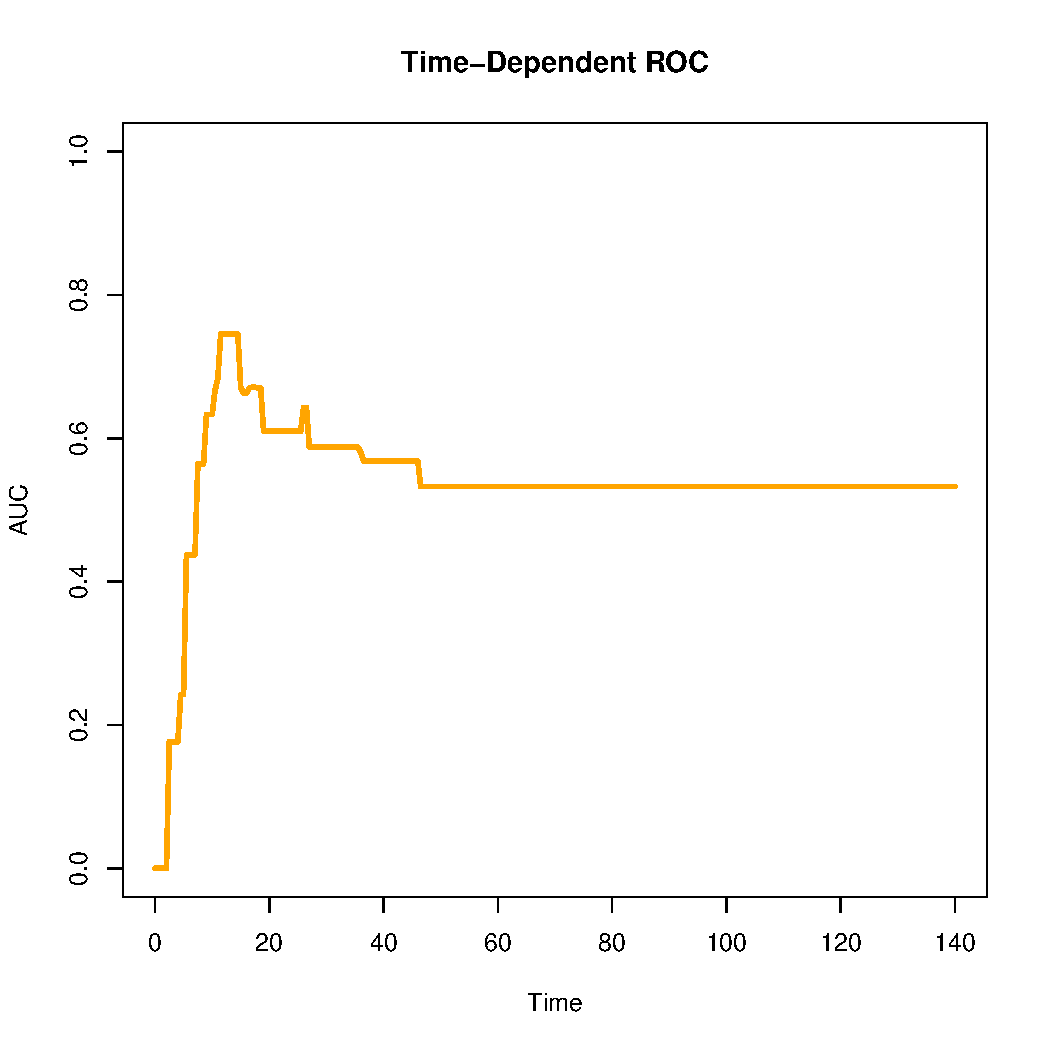
\includegraphics[scale=.4]{raw/pcaAUC.pdf}
      \end{figure}

    }



%  \section{Models}
%    \frame{
%      \frametitle{Model}
%      Model framework assessment \\
%      KM plots as exploration tool \\
%      median survival (w/ CI's) \\
%      Advantages, Disadvantages, and overall idea \\
%      Model selection explanation (Model Assumptions met?)\\
%      interaction terms? \\
%      model fit assessment: deviance residuals, interpretation \\
%
%    }
%
%
%  \section{Results}
%     \frame{
%      \frametitle{Results}
%       Clear presentation of results \\
%       Clear INTERPRETATION of results \\
%       Summary Figures \\
%       Is there any agreement in the model? \\
%       Did some variables show up more than the others? \\
%       show table, graph, list etc\\
%       What variables did not show up? \\
%       Risk scores, curves, KM curves etc \\
%    }

  \section{Comparison of Methods}
    \frame{
      \frametitle{Comparison of Methods}
      \begin{figure}
        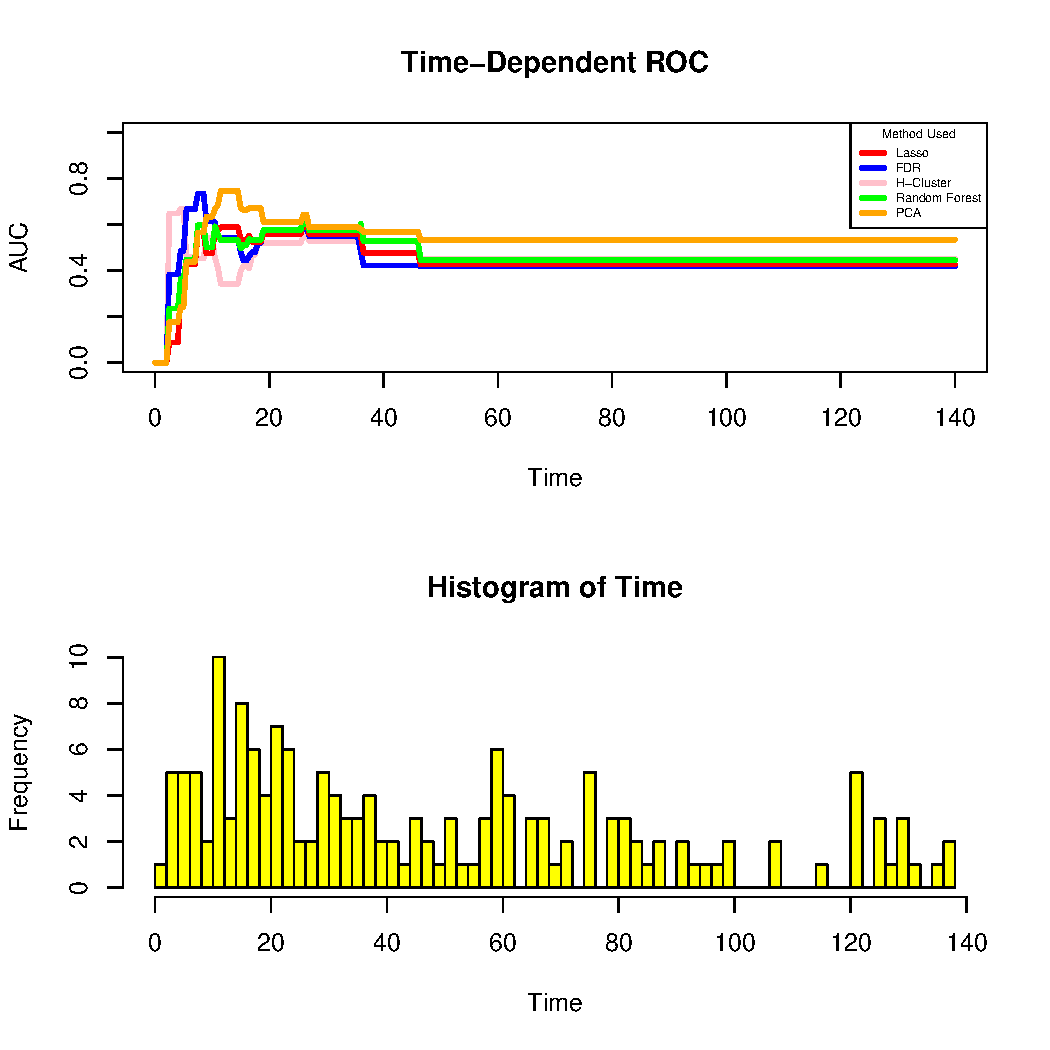
\includegraphics[scale=.4]{raw/finalPlot.pdf}
      \end{figure}
      %Did one model outperform others for all class\\
    }
    
    \frame{
      \frametitle{Covariates that appeared most frequently}
      % latex table generated in R 3.0.3 by xtable 1.7-1 package
% Tue Apr 22 11:34:41 2014
\begin{table}[ht]
\centering
\begin{tabular}{rlllll}
  \hline
 & FDR & Lasso & RF & H-Clust & PCA \\ 
  \hline
ILMN\_1702933 & * & * & * & . & . \\ 
  ILMN\_1689037 & * & * & * & . & . \\ 
  ILMN\_1651611 & . & . & . & * & * \\ 
  ILMN\_1651574 & . & . & . & * & * \\ 
  ILMN\_1651429 & . & . & . & * & * \\ 
  %ILMN\_1889811 & * & . & . & . & . \\ 
  %ILMN\_1809336 & * & . & . & . & . \\ 
  %ILMN\_1807525 & * & . & . & . & . \\ 
  %ILMN\_1767685 & * & . & . & . & . \\ 
  %ILMN\_1757351 & * & . & . & . & . \\ 
  %ILMN\_1749989 & . & . & * & . & . \\ 
  %ILMN\_1745238 & * & . & . & . & . \\ 
  %ILMN\_1718866 & * & . & . & . & . \\ 
  %ILMN\_1714592 & * & . & . & . & . \\ 
  %ILMN\_1714118 & * & . & . & . & . \\ 
  %ILMN\_1704154 & . & . & * & . & . \\ 
  %ILMN\_1690017 & * & . & . & . & . \\ 
  %ILMN\_1666893 & * & . & . & . & . \\ 
  %ILMN\_1651872 & . & . & . & . & * \\ 
  %ILMN\_1651832 & . & . & . & . & * \\ 
  %ILMN\_1651799 & . & . & . & * & . \\ 
  %ILMN\_1651789 & . & . & . & . & * \\ 
  %ILMN\_1651776 & . & . & . & . & * \\ 
  %ILMN\_1651745 & . & . & . & . & * \\ 
  %ILMN\_1651694 & . & . & . & * & . \\ 
  %ILMN\_1651652 & . & . & . & * & . \\ 
  %ILMN\_1651557 & . & . & . & * & . \\ 
  %ILMN\_1651544 & . & . & . & . & * \\ 
  %ILMN\_1651538 & . & . & . & . & * \\ 
  %ILMN\_1651517 & . & . & . & . & * \\ 
  %ILMN\_1651496 & . & . & . & . & * \\ 
  %ILMN\_1651438 & . & . & . & * & . \\ 
  %ILMN\_1651433 & . & . & . & * & . \\ 
  %ILMN\_1651428 & . & . & . & . & * \\ 
  %ILMN\_1651375 & . & . & . & . & * \\ 
  %ILMN\_1651364 & . & . & . & . & * \\ 
  %ILMN\_1651336 & . & . & . & . & * \\ 
  %ILMN\_1651260 & . & . & . & * & . \\ 
  %ILMN\_1651254 & . & . & . & . & * \\ 
  %ILMN\_1651237 & . & . & . & . & * \\ 
  %ILMN\_1651236 & . & . & . & * & . \\ 
   \hline
\end{tabular}
\end{table}

    }

  \section{Future}
    \frame{
      \frametitle{Future}
      Include other covariates
    }

\end{document}
